%% Contrôle recto-verso, deux compétences (Mesurer et construire un angle).
%% Recto : mesurer un angle au rapporteur ; verso : construire un angle de mesure donnée.
%% Figures en VRAIE GRANDEUR : imprimer à 100 %, sans « ajuster à la page ».
%% Tolérance conseillée à la correction : 2° (mesures et constructions).
%% POUR LE CORRIGÉ : remplacer \corrigefalse par \corrigetrue (dans \begin{document}).

%% Font size %%
\documentclass[11pt]{article}

%% Load the custom package
\usepackage{Mathdoc}
\usetikzlibrary{calc}

%% Numéro de séquence %% Titre de la séquence %%
\renewcommand{\centerhead}{S04 - Éval : Mesurer et construire un angle}

%% Spacing commands %%
\renewcommand{\baselinestretch}{1} \setlength{\parindent}{0pt}

\newif\ifcorrige
% Réponse dans une case de largeur fixe : pointillés / réponse en rouge
\newcommand{\rep}[2][1.2cm]{\makebox[#1]{\ifcorrige\textcolor{red}{\textbf{#2}}\else\dotfill\fi}}
% Réponse rédigée sur une ligne : \ligne{réponse}
\newcommand{\ligne}[1]{\makebox[\linewidth][l]{\rule{0pt}{3ex}\ifcorrige\textcolor{red}{#1}\else\dotfill\fi}}
% Croix sur un point
\newcommand{\croix}[1]{\draw #1 ++(-2pt,-2pt) -- ++(4pt,4pt) ++(-4pt,0) -- ++(4pt,-4pt);}

% ---- Recto : angle à mesurer, dans une case de 4,5 cm x 3 cm ----
% \caseMes{sommet x,y}{mesure}{orientation du 1er côté}{L1}{V}{L2}
% Côtés de 2,4 cm (l'élève peut les prolonger).
\newcommand{\caseMes}[6]{%
  \begin{tabular}{@{}c@{}}
  \begin{tikzpicture}
    \useasboundingbox (0,0) rectangle (4.5,2.75);
    \begin{scope}[shift={(#1)}]
      \draw[thick] (#3:2.4) -- (0,0) -- ({#3+#2}:2.4);
      \croix{(#3:2.1)} \croix{({#3+#2}:2.1)}
      \node at ($(#3:2.1)+({#3-90}:3mm)$) {$#4$};
      \node at ({#3+#2/2+180}:3.5mm) {$#5$};
      \node at ($({#3+#2}:2.1)+({#3+#2+90}:3mm)$) {$#6$};
    \end{scope}
  \end{tikzpicture}\\
  $\widehat{#4#5#6} = $ \rep{#2}$\degre$
  \end{tabular}}
% Case exemple (mesure déjà donnée, fond grisé)
\newcommand{\caseMesEx}[6]{%
  \colorbox{gray!15}{\begin{tabular}{@{}c@{}}
  \begin{tikzpicture}
    \useasboundingbox (0,0) rectangle (4.3,2.65);
    \begin{scope}[shift={(#1)}]
      \draw[thick] (#3:2.4) -- (0,0) -- ({#3+#2}:2.4);
      \croix{(#3:2.1)} \croix{({#3+#2}:2.1)}
      \node at ($(#3:2.1)+({#3-90}:3mm)$) {$#4$};
      \node at ({#3+#2/2+180}:3.5mm) {$#5$};
      \node at ($({#3+#2}:2.1)+({#3+#2+90}:3mm)$) {$#6$};
    \end{scope}
  \end{tikzpicture}\\
  \textit{Ex.} : $\widehat{#4#5#6} = #2\degre$
  \end{tabular}}}

% Rapporteur (centre à l'origine, rayon 3,3 avant mise à l'échelle) :
% graduation extérieure : 0 à droite ; graduation intérieure : 0 à gauche.
\newcommand{\rapporteur}{%
  \fill[blue!4] (3.3,0) arc[start angle=0, end angle=180, radius=3.3] -- cycle;
  \draw[blue!60!black] (3.3,0) arc[start angle=0, end angle=180, radius=3.3] -- cycle;
  \draw[blue!60!black] (2.1,0) arc[start angle=0, end angle=180, radius=2.1];
  \foreach \t in {0,5,...,180} \draw[blue!60!black] (\t:3.3) -- (\t:3.15);
  \foreach \t in {0,10,...,180} {
    \draw[blue!60!black] (\t:3.3) -- (\t:3.0);
    \node[blue!60!black, font=\fontsize{4.5pt}{5pt}\selectfont, inner sep=0pt, rotate=\t-90] at (\t:2.8) {\t};
    \pgfmathtruncatemacro{\u}{180-\t}
    \node[blue!60!black, font=\fontsize{4.5pt}{5pt}\selectfont, inner sep=0pt, rotate=\t-90] at (\t:2.45) {\u};
  }
  \draw[blue!60!black] (-0.15,0) -- (0.15,0) (0,0) -- (0,0.15);
}

% ---- Verso : demi-droite donnée, angle à construire ----
% \caseConstr{largeur}{hauteur}{sommet x,y}{direction du côté donné}{longueur}{mesure}{sens (1 direct, -1 indirect)}{sommet}{pt du côté donné}{nom du pt construit}
\newcommand{\caseConstr}[9]{%
  \begin{tikzpicture}
    \useasboundingbox (0,0) rectangle (#1);
    \begin{scope}[shift={(#2)}]
      \draw[thick] (0,0) -- (#3:#4);
      \croix{(#3:{#4-0.4})}
      \node at ($(#3:{#4-0.4})+({#3-90*#6}:3.5mm)$) {$#8$};
      \node at ({#3+#6*#5/2+180}:4mm) {$#7$};
      \ifcorrige
        \begin{scope}[red]
          \draw (0,0) -- (#3:6mm) arc[start angle=#3, delta angle={#6*#5}, radius=6mm] -- cycle;
          \draw[thick] (0,0) -- ({#3+#6*#5}:4);
          \croix{({#3+#6*#5}:3.5)}
          \node at ($({#3+#6*#5}:3.5)+({#3+#6*#5+90*#6}:3.5mm)$) {$#9$};
          \node at ({#3+#6*#5/2}:1.15) {\small $#5\degre$};
        \end{scope}
      \fi
    \end{scope}
  \end{tikzpicture}}

\newcommand{\bandeau}[3][]{\noindent\colorbox{gray!15}{\parbox{\dimexpr\linewidth-2\fboxsep}{\textbf{Compétence #2 : #3}\hfill\textit{\small #1}}}\par}

\newcommand{\feuille}{%
\phantom{0}
\vspace{-.5cm}

\entetedevoirs{40}
\enlargethispage{8mm}

\vspace{-2mm}
{\small\competences{
6C04-GEO14 & Mesurer un angle au rapporteur & & & & \\ \hline
6C04-GEO15/16 & Construire un angle de mesure donnée & & & & \\ \hline
}}

\smallskip
\begin{center}
\textit{Durée : 35 minutes \quad -- \quad Total : 40 points \quad -- \quad Calculatrice non autorisée.}\\
\textit{Matériel : rapporteur, règle, crayon bien taillé.}
\end{center}

\vspace{-3mm}
\bandeau[Tu peux prolonger les côtés.]{6C04-GEO14}{Mesurer un angle au rapporteur}
\vspace{-0.5cm}
% Mesures : ex. 50 | a 35 | b 120 | c 75 | d 130 | e 65 | f 25 | g 105
\begin{exercicedevoir}[7][Mesure les angles]
\vspace{-0.3cm}
Mesure chaque angle avec ton rapporteur, comme dans l'exemple. \hfill \textit{\small (1 point par angle)}

\setlength{\tabcolsep}{0pt}
\begin{tabularx}{\textwidth}{@{}*{4}{>{\centering\arraybackslash}X}@{}}
\caseMesEx{0.6,0.3}{50}{0}{A}{B}{C} &
\caseMes{0.5,0.2}{35}{15}{D}{E}{F} &
\caseMes{2.2,0.25}{120}{30}{G}{H}{I} &
\caseMes{3.2,0.3}{75}{100}{J}{K}{L} \\[4mm]
\caseMes{2.25,0.3}{130}{25}{M}{N}{P} &
\caseMes{3.3,2.3}{65}{200}{R}{S}{T} &
\caseMes{3.6,0.4}{25}{140}{U}{V}{W} &
\caseMes{3.2,2.35}{105}{190}{X}{Y}{Z} \\
\end{tabularx}
\end{exercicedevoir}

\vspace{-0.85cm}
% Triangle : A = 40°, B = 65°, C = 75° (réduit : seules les mesures d'angles comptent)
\begin{exercicedevoir}[6][Dans un triangle]
\vspace{-0.3cm}
\begin{minipage}[c]{0.4\linewidth}\centering
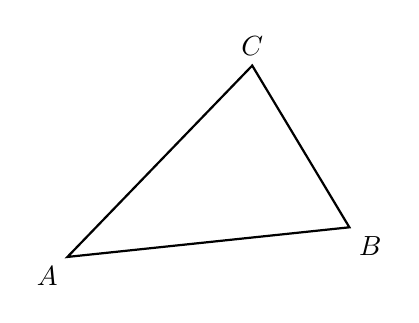
\begin{tikzpicture}[rotate=6, scale=0.6]
  \coordinate (A) at (0,0); \coordinate (B) at (6,0); \coordinate (C) at (40:5.63);
  \draw[thick] (A) -- (B) -- (C) -- cycle;
  \node[below left] at (A) {$A$}; \node[below right] at (B) {$B$}; \node[above] at (C) {$C$};
\end{tikzpicture}
\end{minipage}\hfill
\begin{minipage}[c]{0.57\linewidth}
Mesure les trois angles du triangle $ABC$.\\ \textit{\small (2 points par angle)}

\renewcommand{\arraystretch}{1.8}
\begin{tabular}{@{}lll@{}}
$\widehat{BAC} = $ \rep{40}$\degre$ \quad & $\widehat{ABC} = $ \rep{65}$\degre$ \quad & $\widehat{ACB} = $ \rep{75}$\degre$ \\
\end{tabular}
\end{minipage}
\end{exercicedevoir}

\vspace{-0.85cm}
% Rapporteur : [Oy) sur le 0 de la graduation intérieure, angle xOy = 40°
\begin{exercicedevoir}[7][Lire le rapporteur]
\vspace{-0.3cm}
\begin{minipage}[c]{0.42\linewidth}\centering
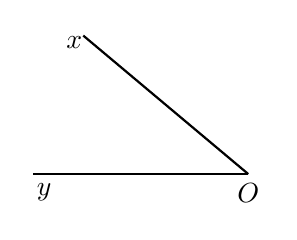
\begin{tikzpicture}[scale=0.72]
  \rapporteur
  \draw[thick] (0,0) -- (-3.8,0);
  \draw[thick] (0,0) -- (140:3.8);
  \croix{(-3.6,0)} \node[below] at (-3.6,0) {$y$};
  \croix{(140:3.6)} \node[left] at (140:3.6) {$x$};
  \node[below] at (0,0) {$O$};
\end{tikzpicture}
\end{minipage}\hfill
\begin{minipage}[c]{0.55\linewidth}
\textbf{a.} Quelle est la mesure de l'angle $\widehat{xOy}$ ? \hfill \textit{\small (2 points)}\\[1mm]
$\widehat{xOy} = $ \rep{40}$\degre$

\smallskip
\textbf{b.} Tom a lu $140\degre$. Explique son erreur. \hfill \textit{\small (3 points)}
\ligne{Le côté $[Oy)$ est sur le 0 de la graduation intérieure :}
\ligne{il fallait lire la graduation intérieure, pas l'extérieure.}

\smallskip
\textbf{c.} Nature de l'angle $\widehat{xOy}$ : \rep[2cm]{aigu} \hfill \textit{\small (2 points)}
\end{minipage}
\end{exercicedevoir}

\newpage
\bandeau[Place bien le centre du rapporteur.]{6C04-GEO15/16}{Construire un angle de mesure donnée}
\vspace{-0.5cm}
\begin{exercicedevoir}[6][Construis l'angle]
\vspace{-0.3cm}
Construis l'angle demandé à partir de la demi-droite déjà tracée. Place le point $y$ sur le côté que tu traces. \hfill \textit{\small (2 points par angle)}

\smallskip
\setlength{\tabcolsep}{0pt}
\begin{tabularx}{\textwidth}{@{}*{3}{>{\centering\arraybackslash}X}@{}}
\caseConstr{5.8,4.4}{0.4,0.4}{0}{4.5}{40}{1}{O}{x}{y} &
\caseConstr{5.8,4.4}{2.4,0.4}{0}{3.2}{115}{1}{O}{x}{y} &
\caseConstr{5.8,4.4}{5.3,0.4}{180}{4.8}{70}{-1}{O}{x}{y} \\
a) $\widehat{xOy} = 40\degre$ & b) $\widehat{xOy} = 115\degre$ & c) $\widehat{xOy} = 70\degre$ \\
\end{tabularx}
\end{exercicedevoir}

\vspace{-0.85cm}
\begin{exercicedevoir}[6][Un côté penché]
\vspace{-0.3cm}
Construis l'angle demandé à partir de la demi-droite déjà tracée. \hfill \textit{\small (3 points par angle)}

\smallskip
\setlength{\tabcolsep}{0pt}
\begin{tabularx}{\textwidth}{@{}*{2}{>{\centering\arraybackslash}X}@{}}
\caseConstr{8,4.6}{1.2,0.4}{25}{5}{60}{1}{A}{B}{C} &
\caseConstr{8,4.6}{4.6,0.6}{160}{4.6}{125}{-1}{E}{D}{F} \\
a) $\widehat{BAC} = 60\degre$ & b) $\widehat{DEF} = 125\degre$ \\
\end{tabularx}
\end{exercicedevoir}

\vspace{-0.85cm}
% Triangle RST : RS = 6 cm, SRT = 45°, RST = 80° donc RTS = 55° (RT = 7,21 cm)
\begin{exercicedevoir}[8][Construis un triangle]
\vspace{-0.3cm}
\begin{minipage}[c]{0.5\linewidth}\centering
\begin{tikzpicture}
  \useasboundingbox (-0.5,-0.5) rectangle (7,5.6);
  \coordinate (R) at (0,0); \coordinate (S) at (6,0); \coordinate (T) at (45:7.21);
  \draw[thick] (R) -- (S);
  \node[below left] at (R) {$R$}; \node[below right] at (S) {$S$};
  \ifcorrige
    \begin{scope}[red]
      \draw[thick] (R) -- (T) -- (S);
      \draw (R) -- (6mm,0) arc[start angle=0, end angle=45, radius=6mm] -- cycle;
      \draw (S) -- ++(-6mm,0) arc[start angle=180, end angle=100, radius=6mm] -- cycle;
      \node[above] at (T) {$T$};
      \node at (22.5:1.1) {\small $45\degre$};
      \node at ($(S)+(140:1.1)$) {\small $80\degre$};
    \end{scope}
  \fi
\end{tikzpicture}
\end{minipage}\hfill
\begin{minipage}[c]{0.47\linewidth}
Le segment $[RS]$ mesure $6$ cm.

\smallskip
\textbf{a.} Construis le triangle $RST$ tel que\\
$\widehat{SRT} = 45\degre$ et $\widehat{RST} = 80\degre$. \hfill \textit{\small (4 points)}

\medskip
\textbf{b.} Mesure l'angle $\widehat{RTS}$ :\\
$\widehat{RTS} = $ \rep{55}$\degre$ \hfill \textit{\small (2 points)}

\medskip
\textbf{c.} Quelle est la nature de l'angle $\widehat{RST}$ ?\\
\rep[2cm]{aigu} \hfill \textit{\small (2 points)}
\end{minipage}
\end{exercicedevoir}
}

\begin{document}

\corrigefalse
\feuille

\end{document}

%%% Local Variables:
%%% mode: LaTeX
%%% TeX-master: t
%%% End:
